\documentclass{article}

%
% Importering av pakker
%
\usepackage{pgf,pgfarrows,pgfnodes}
\usepackage{tikz}
\usepackage{braket}
\usetikzlibrary{arrows,backgrounds,shapes.geometric,shadows}
\bibliographystyle{plain}
\usepackage[text={7in,9in},centering]{geometry}
\usepackage{amsbsy, amsfonts}
\usepackage{mathtools}


\usepackage{lmodern}
\usetikzlibrary{external}
\usetikzlibrary{arrows}
\usetikzlibrary{decorations.pathmorphing}

\tikzset{snake it/.style={decorate, decoration=snake}}
\tikzexternalize

\begin{document}
\vspace*{2cm}
\begin{center}
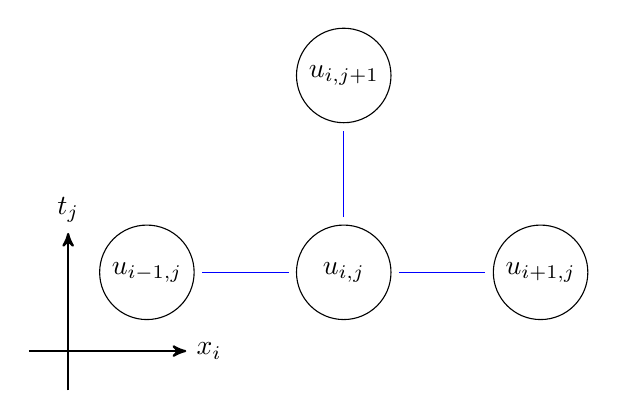
\begin{tikzpicture}[
    axis/.style={thick, ->, >=stealth'},
    important line/.style={thick},
    dashed line/.style={dashed, thin},
    pile/.style={thick, ->, >=stealth', shorten <=2pt, shorten
    >=2pt},
    every node/.style={color=black}
    ]

\draw[axis] (-4.0,-1.0)  -- (-2.0,-1.0) node(xline)[right]
        {$x_i$};
    \draw[axis] (-3.5,-1.5) -- (-3.5,0.5) node(yline)[above] {$t_j$};

\draw (0,0) circle (0.6) node {$u_{i,j}$};

\draw (2.5,0) circle (0.6) node {$u_{i+1,j}$};

\draw (-2.5,0) circle (0.6) node {$u_{i-1,j}$};

\draw (0,2.5) circle (0.6) node {$u_{i,j+1}$};

\path [draw=blue]
    (0.7,0.0) -- (1.8,0.0);

\path [draw=blue]
    (-0.7,0.0) -- (-1.8,0.0);

\path [draw=blue]
    (0.0,0.7) -- (0.0,1.8);
    
\end{tikzpicture}
\end{center}
\end{document}